\documentclass{article}
\usepackage[margin=1in]{geometry}
\usepackage{microtype}
\usepackage{setspace}
\usepackage{amsmath}
\usepackage{parskip}
\usepackage{amssymb}
\usepackage{graphicx}

\graphicspath{{../public/}}

\parskip=4ex
\date{}
\author{}

\title{10.7 Vector Functions and Space Curves}

\begin{document}
  \maketitle
  A vector-valued function or vector function is a function whose domain is a seet of real numbers and whose range is a set of vectors. If $ f(t), g(t) ~\&~ h(t) $ are the component vector $ r(t) $, then $ f,g,~\&~ h $ are real-valued functions called the component functions of $ r $. Due to this we can write
  \[
    \begin{gathered}
    r(t)=< f(t), g(t), h(t)>=f(t)i + g(t)j + h(t)k 
    \end{gathered}
  \]

  \textbf{Ex 1}\\
  If
  \[
    r(t)=< t^{3}, ln(3-t), \sqrt{t}> 
  \]
  then the component functions are
  \[
    f(t)=t^{3} \qquad g(t)=ln(3-t) \qquad h(t)=\sqrt{t}  
  \]
 
  The domain of $ r $ are all values of $ t $ for which the expression for $ r(t) $ is defined. We can see that $ r(t) $ is defined when
  \[
    \begin{gathered}
      3-t>0 ~\&~t\ge 0 \to \{t|0\le t <3\} \to [0,3)
    \end{gathered}
  \]
 
  \textbf{Limit of Vector Functions}\\
  The limit of a vector function $ r $ is defined by taking the limits of its component functions. 

  Given the vector function, $r(t)=< f(t), g(t), h(t)>$, we can take the limit of it like so
  \[
    \begin{gathered}
    \lim_{ t \to a}{r(t)}= < \lim_{t \to a}{f(t)}, \lim_{t \to a}{g(t)}, \lim_{t \to a}{h(t)}  
    \end{gathered}
  \]
  provided that the limits of the component functions exist.

  If $ \lim_{t \to a}{r(t)} = \mathcal{L} $, this definition is equal to saying that the length and direction of the vector $ r(t) $ approach the length and direction of the vector $ \mathcal{L} $.
 
  \textbf{Ex 2}
  Find $ \lim_{t \to 0}{r(t)} $, where $ r(t)=(1+t^{3})i + te^{-t}j + \frac{\sin{t}}{t}k$ 
  \[
      \begin{gathered}
        \lim_{t \to 0}{r(t)}= \text{\large{[}} \lim_{t \to 0}{(1+t^{3} )} \text{\large{]}}i + \text{\large{[}} \lim_{t \to 0}{te^{-t} } \text{\large{]}}j + \text{\large{[}} \lim_{t \to 0}{\frac{\sin{t}}{t} } \text{\large{]}}k \to \boxed{i+k}
      \end{gathered}
  \]
 
  A vector function $ r $ is continuous at a if
  \[
    \lim_{t \to a}{r(t)}=r(a)
  \]
  
  Due to this then $ r $ is continuous at $ a $ if and only if its component functions $ f,g ~\&~ h $ are continuous at $ a $.

  There is a connection between continuous vector functions and space curves. Suppousing that $ f,g ~\&~ h $ are continuous real-valued functions on an interval $ I $. Then the set $ C $ of all points $ (x,y,z) $ in space, where
  \[
      x=f(t) \qquad y=g(t) \qquad z=h(t)
  \]
  and $ t $ varies throughout the interval $ I $, is called a space curve. Imagine $ C $ as being traced out by a moving particle whose position at time $ t $ is $ < f(t), g(t), h(t) >  $. Then it can be said that $ r(t) $ is the position vector of the point $ P(f(t),g(t),h(t)) $.
  \begin{center}
      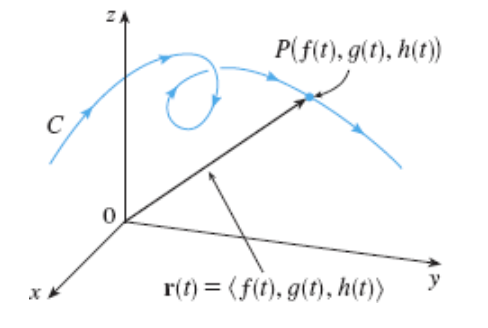
\includegraphics[width=8cm]{c_trace}
  \end{center}

  $ C $ is traced out by the tip of a moving position vector $ r(t) $.

  \textbf{Ex 5}\\
  Find a vector equation and parametric equations for the line segment that joins the point $ P(1,3,-2) $ to the point $ Q(2,-1,3) $.
  \[
    \begin{gathered}
      r(t)=(1-t)r_{0}+tr_{1}~0\let\le1\\
      ~\\
      r(t)=(1-t)< 1, 3, -2 > +t< 2, -1, 3 > ~0\le t \le 1\\
      ~\\
     r(t) = < t+1, -4t+3, 5t-2 >\\
     ~\\
     x=t+1 \qquad y=-4t+3 \qquad z=5t-2~0\le t \le 1
    \end{gathered}
  \]

  \textbf{Ex 6}\\
  Find a vector function that represents the curve of intersection of the cylinder $ x^{2}+y^{2}+1$ and the plane $ y+z $=2
  \begin{center}
      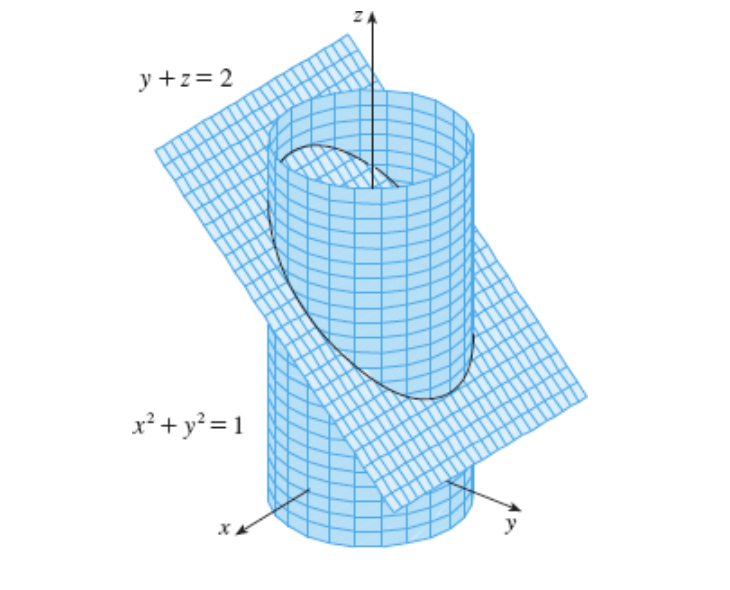
\includegraphics[width=6cm]{10_7_1}
      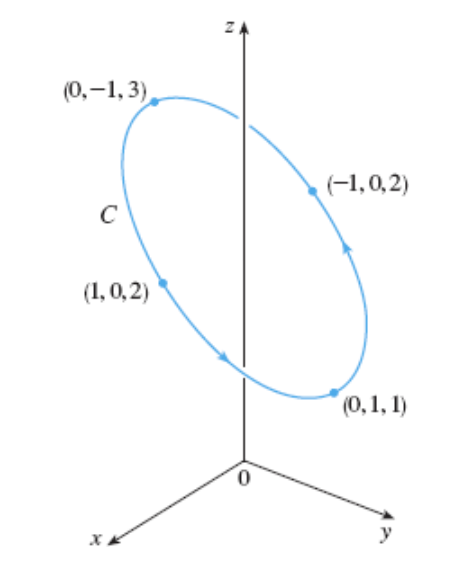
\includegraphics[width=4cm]{10_7_2}
  \end{center}
  Figure 5 (LHS) shows the intersection of the plane and cylinder. While Figure 6 (RHS) shows the curve of intersection $ C $, which is an eclipse.

  The projection of $ C $ onto the xy plane is the circle $ x^{2}+y^{2=1}$, $ z=0 $. So we can rewrite the equation like so   
  \[
      \begin{gathered}
        x^{2}+y^{2}=1,~z=0 \to \sin^{2}{t}+\cos^{2}{t}=1\\
        ~\\
        x=\sin{t} \qquad y=\cos{t} \qquad 0\le t \le 2\pi\\
        ~\\
        y+z=2 \to z=2-y \to z = 2 - \cos{t}\\
        ~\\
        C: x=\sin{t} \qquad y=\cos{t} z = 2-\cos{t}\\
        ~\\
        r(t)=\sin{t}i+\cos{t}k+(2-\cos{t})k \qquad 0\le t \le 2\pi
      \end{gathered}
  \]

  \textbf{Derivatives}\\
  The derivative $ r' $ of a vector function $ r $ is defined in much the same way as for real-valued functions:
  \[
      \begin{gathered}
      \frac{dr}{dt} =r'(t)=\lim_{h \to 0}{\frac{r(t+h)-r(t)}{h}}
      \end{gathered}
  \]
  if this limit exists. The geometric signifance of this is shown below.
  \begin{center}
      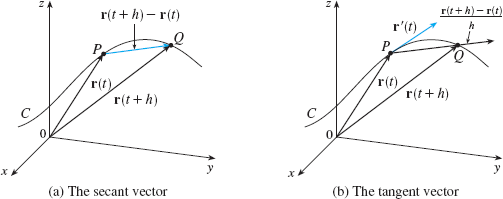
\includegraphics[width=12cm]{10_7_3}
  \end{center}

  There exists a tangent vector, $ r'(t) $, to the curve defined by $ r $ at the point $ P $, provided that $ r'(t) ~\&~ r'(t) \neq 0$. The tangent line to $ C $ at $ P $ is defined to be the line through $ P $ parallel to the tangent vector $ r'(t) $. There is also the unit tangent vector
  \[
      T(t)=\frac{r'(t)}{| r'(t) |} 
  \]

  The reason that the tangent vector $r'(t)$ at the point $ P $ is parallel to its tangent line is because the derivative gives us the instantaneuous rate of change at a point. By finding the derivative of a vector equation at a point $ P $, we are finding the instant rate of change as a vector. Since the tangent vector is the slope of the tangent line, the tangent vector is parallel to the direction of the tangent line.
  \[
      r(t)=r_{0}+tv\to \gamma(t)=P + t \cdot r'(t)
  \]

  \textbf{Theorem}\\
  If $ r(t) =< f(t), g(t), h(t) > = f(t)i + g(t)j + h(t)k$, where $ f,g,~\&~ h $ are differentiable functions, then
  \[
    r'(t) =< f'(t), g'(t), h'(t) > = f'(t)i + g'(t)j + h'(t)k
  \]

  \textbf{Ex 8A}\\
  Find the derivative of $ r(t) =(1+t^{3})i+te^{-t}j+\sin{2t}k$
  \[
      \begin{gathered}
        \boxed{r'(t)=3t^{2}+(1-t)e^{-t}+2\cos{2t}k} 
      \end{gathered}
  \]

  \textbf{Ex 8B}\\
  Find the unit tangent vector at the point where $ t=0 $
  \[
      \begin{gathered}
      r'(0)\to j +2k>\\
      ~\\
    T(0)=\frac{r'(0)}{| r'(0) |}=\frac{j+2k}{\sqrt{5}}=\boxed{\frac{1}{\sqrt{5}}j+\frac{2}{\sqrt{5}}k} 
      \end{gathered}
  \]

  \textbf{Ex 10}\\
  Find parametric equations of the tangent line to the helix, $ x=2\cos{t},y=\sin{t},~\&~ z=t$,  with parametric equations at the point $ (0,1,\frac{\pi}{2}) $.
  \[
      \begin{gathered}
      r(t)=< 2\cos{t}, \sin{t}, t >\\
      ~\\
      r'(t)=< -2\sin{t}, \cos{t}, 1 >\\
      ~\\
      t=\frac{\pi}{2}\\
      ~\\
      r'(\frac{\pi}{2})=< -2, 0, 1 > 
      \end{gathered}
  \]

  The tangent line is through $ (0,1,\frac{\pi}{2}) $ parallel to the vector $ < -2, 0, 1 >$ so
  \[
      \begin{gathered}
      tv=t \cdot r'(\frac{\pi}{2}) = t< -2, 0, 1 > = < -2, 0, t >\\
      ~\\
      x=-2t \qquad y=1 \qquad z=t+\frac{pi}{2}  
      \end{gathered}
  \]

  \textbf{Differentiation Rules}\\
  Suppouse $ \vec{u} ~\&~ \vec{v} $ are different vector functions, $ c $ is a scalar and $ f $is a real valued function.
  \[
      \begin{aligned}
      &1)~\frac{d}{dt} \text{\large{[}} \vec{u}(t)+\vec{v}(t) \text{\large{]}}=\vec{u'}(t)+\vec{v'}(t)\\
      ~\\
      &2)~\frac{d}{dt} \text{\large{[}} c\vec{u}(t) \text{\large{]}}=c\vec{u'}(t)\\
      ~\\
      &3)~\frac{d}{dt} \text{\large{[}} f(t) \cdot \vec{u}(t) \text{\large{]}}=f'(t)\cdot \vec{u}(t)+f(t)\cdot \vec{u'}(t)\\
      ~\\
      &4)~\frac{d}{dt} \text{\large{[}} \vec{u}(t) \cdot \vec{v}(t) \text{\large{]}}=\vec{u'}(t) \cdot \vec{v}(t)+\vec{u}(t)\cdot \vec{v'}(t)
      ~\\
      &5)~\frac{d}{dt} \text{\large{[}} \vec{u}(t) \times \vec{v}(t) \text{\large{]}}=\vec{u'}(t) \times \vec{v}(t) + \vec{u}(t) \times \vec{v'}(t)\\
      ~\\
      &6)~\frac{d}{dt} \text{\large{[}} \vec{u}(f(t)) \text{\large{]}}=f'(t) \cdot \vec{u'}(f(t))
      \end{aligned}
  \]

  \textbf{Definite Integral}\\
  If $ \vec{r}(t) $ is a continuous vector function with components
  \[
      \begin{gathered}
      r(t)=< f(t), g(t), h(t) >\\
      ~\\
      \int^{b}_{a} r(t)~dt \to \text{\large{(}} \int^{b}_{a} f(t)~dt \text{\large{)}}i + \text{\large{(}} \int^{b}_{a} g(t)~dt \text{\large{)}}j + \text{\large{(}} \int^{b}_{a} h(t)~dt \text{\large{)}}k\\
      \end{gathered}
  \]
  As shown, evaluating the integral of a vector function is done so by integrating each component function, $ < x, y, z >  $. The Fundamental Theorem of Calculus applies here as well as shown below.
  \[
      \int^{b}_{a} r(t)~dt=R(t) \text{\large{]}}^{b}_{a}=R(b) -R(a)
  \]

  Where $ R $ is an antiderivative of $ r $, that is $ R'(t) = r(t)$.

  \textbf{Ex 12}\\
  If $ r(t) =2\cos{t}i+\sin{t}j+2tk$, then
  \[
      \begin{gathered}
      \int r(t)~dt= \text{\large{(}} \int 2\cos{t}~dt \text{\large{)}}i+ \text{\large{(}} \int \sin{t}~dt \text{\large{)}}j + \text{\large{(}} \int 2t~dt \text{\large{)}}k\\
      ~\\
      \boxed{\text{\large{(}} 2\sin{t} \text{\large{)}}i - \text{\large{(}} \cos{t} \text{\large{)}}j + 2k + C}\\
      ~\\
      \int^{\frac{\pi}{2}}_{0} r(t)~dt= \text{\large{[}} 2\sin{t}i - \cos{t}j + t^{2}k \text{\large{]}}^{\frac{\pi}{2}}_{0}= \boxed{2i+j+\frac{\pi^{2}}{4}k} 
      \end{gathered}
  \]
  

\end{document}
